\section{Resumen de aprobados}
A la universidad Santa María, lider en ingeniería, magia y hechicería, llegan alumnos de intercambio provenientes de Hogwarts para tomar el curso de defensa contra las artes oscuras. Los profesores (magos) son nulos en el manejo de datos y le piden a los buenos estudiantes de IWI-131 (muggles) que van a los intensivos de CIAC ayuda con el filtro de alumnos aprobados y reprobados. Las reglas para aprobar son:
\begin{itemize}
    \item Que el promedio de sus notas sea mayor o igual a 55.
    \item Que el porcentaje de asistencia sea mayor al 75\%
\end{itemize}

De cumplirse ambas condiciones, el estudiante aprueba, de cumplirse sólo una, el estudiante debe dar un examen global y de no cumplirse ninguna el estudiante reprueba.

Se tienen los archivos: notas.txt y asistencia.txt

\begin{figure}[h]
    \centering
    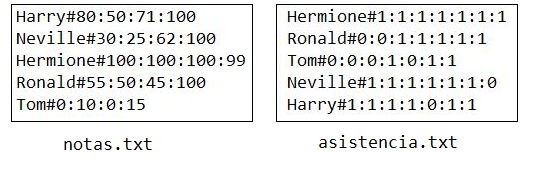
\includegraphics[scale=0.9]{Imagenes/archivos1.jpg}
\end{figure}

El archivo notas.txt tiene la estructura \texttt{nombre\_alumno\#nota1: ... :nota4}, mientras que el archivo asistencia.txt tiene la estructura \texttt{nombre\_alumno\#asis1: ... :asis7}. A usted se le pide:

\begin{itemize}
    \item[a.] Desarrollar la función \texttt{listado\_alumnos(nombre\_archivo)} que reciba como parámetro el nombre de uno de los dos archivos y retorne una lista con todos los alumnos.
    \begin{lstlisting}[style=consola]
>>>listado_alumnos('notas,txt')
['Harry','Neville','Hermione','Ronald','Tom']
    \end{lstlisting}
    \item[b.] Desarrollar la función \texttt{aprueba\_por\_notas(nombre\_archivo)} que reciba como parámetro el nombre del archivo con las notas y retorne un diccionario que asocie el nombre del alumno con un booleano según haya o no cumplido con el requisito número 1.
    \begin{lstlisting}[style=consola]
>>>aprueba_por_notas('notas.txt')
{'Ronald':True,'Neville':False,'Harry':True,'Hermione':True,'Tom':False}
    \end{lstlisting}
    \item[c.] Programar la función \texttt{aprueba\_por\_asistencia(nombre\_archivo)} que reciba como parámetro el nombre del archivo con las asistencias y retorne un diccionario que asocie el nombre del alumno con un booleano según haya o no cumplido con el requisito número 2.
    \begin{lstlisting}[style=consola]
>>>aprueba_por_asistencia('asistencia.txt')
{'Ronald':False,'Neville':True,'Harry':True,'Hermione':True,'Tom':False}
    \end{lstlisting}
    \item[d.] Crear la función \texttt{resumen(archivo\_notas,archivo\_asistencia)} que reciba los nombres de ambos archivos, y cree el archivo \texttt{Final.txt} con la estructura \texttt{nombre\#estado}, donde estado puede ser (APROBADO, EXAMEN GLOBAL, REPROBADO) de cada alumno. La función retorna None.
    \begin{figure}[h]
    \centering
    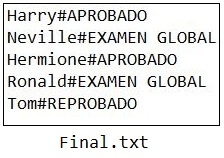
\includegraphics[scale=0.9]{Imagenes/final.jpg}
    \end{figure}
\end{itemize}